

\tikzset{every picture/.style={line width=0.75pt}} %set default line width to 0.75pt        
\resizebox{\textwidth}{!}{%
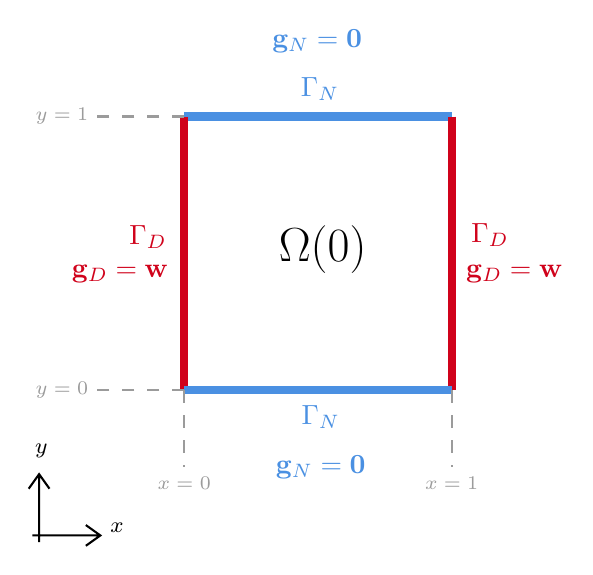
\begin{tikzpicture}[x=0.75pt,y=0.75pt,yscale=-1,xscale=1]
%uncomment if require: \path (0,336); %set diagram left start at 0, and has height of 336

%Straight Lines [id:da3775330886942099] 
\draw [color={rgb, 255:red, 74; green, 144; blue, 226 }  ,draw opacity=1 ][line width=3]    (113.28,81.05) -- (242.14,81.05) ;
%Straight Lines [id:da7311947956092497] 
\draw [color={rgb, 255:red, 208; green, 2; blue, 27 }  ,draw opacity=1 ][line width=3]    (242.14,81.05) -- (242.14,212.95) ;
%Straight Lines [id:da6649609020271117] 
\draw [color={rgb, 255:red, 208; green, 2; blue, 27 }  ,draw opacity=1 ][line width=3]    (113.28,81.05) -- (113.28,212.95) ;
%Straight Lines [id:da0032656115651366058] 
\draw [color={rgb, 255:red, 74; green, 144; blue, 226 }  ,draw opacity=1 ][line width=3]    (242.14,212.95) -- (113.28,212.95) ;
%Shape: Axis 2D [id:dp28368375799841394] 
\draw  (40.08,282.88) -- (72.88,282.88)(43.36,253.36) -- (43.36,286.16) (65.88,277.88) -- (72.88,282.88) -- (65.88,287.88) (38.36,260.36) -- (43.36,253.36) -- (48.36,260.36)  ;

%Straight Lines [id:da4221223762377593] 
\draw [color={rgb, 255:red, 155; green, 155; blue, 155 }  ,draw opacity=1 ] [dash pattern={on 4.5pt off 4.5pt}]  (113.28,212.95) -- (113.28,250) ;
%Straight Lines [id:da5345451203989031] 
\draw [color={rgb, 255:red, 155; green, 155; blue, 155 }  ,draw opacity=1 ] [dash pattern={on 4.5pt off 4.5pt}]  (242.14,212.95) -- (242.14,250) ;
%Straight Lines [id:da5891570191879292] 
\draw [color={rgb, 255:red, 155; green, 155; blue, 155 }  ,draw opacity=1 ] [dash pattern={on 4.5pt off 4.5pt}]  (113.28,212.95) -- (70.5,212.95) ;
%Straight Lines [id:da22019042876536155] 
\draw [color={rgb, 255:red, 155; green, 155; blue, 155 }  ,draw opacity=1 ] [dash pattern={on 4.5pt off 4.5pt}]  (113.28,81.05) -- (70.5,81.05) ;

% Text Node
\draw (106.32,138.93) node [anchor=east] [inner sep=0.75pt]  [color={rgb, 255:red, 208; green, 2; blue, 27 }  ,opacity=1 ]  {$\Gamma _{D}$};
% Text Node
\draw (250.14,138.04) node [anchor=west] [inner sep=0.75pt]  [color={rgb, 255:red, 208; green, 2; blue, 27 }  ,opacity=1 ]  {$\Gamma _{D}$};
% Text Node
\draw (178.66,74.95) node [anchor=south] [inner sep=0.75pt]  [color={rgb, 255:red, 74; green, 144; blue, 226 }  ,opacity=1 ]  {$\Gamma _{N}$};
% Text Node
\draw (179.09,218.96) node [anchor=north] [inner sep=0.75pt]  [color={rgb, 255:red, 74; green, 144; blue, 226 }  ,opacity=1 ]  {$\Gamma _{N}$};
% Text Node
\draw (107.05,150.96) node [anchor=north east] [inner sep=0.75pt]  [color={rgb, 255:red, 208; green, 2; blue, 27 }  ,opacity=1 ]  {$\mathbf{g}_{D} =\mathbf{w}$};
% Text Node
\draw (247.65,150.96) node [anchor=north west][inner sep=0.75pt]  [color={rgb, 255:red, 208; green, 2; blue, 27 }  ,opacity=1 ]  {$\mathbf{g}_{D} =\mathbf{w}$};
% Text Node
\draw (179.08,242.86) node [anchor=north] [inner sep=0.75pt]  [color={rgb, 255:red, 74; green, 144; blue, 226 }  ,opacity=1 ]  {$\mathbf{g}_{N} =\mathbf{0}$};
% Text Node
\draw (177.35,51.93) node [anchor=south] [inner sep=0.75pt]  [color={rgb, 255:red, 74; green, 144; blue, 226 }  ,opacity=1 ]  {$\mathbf{g}_{N} =\mathbf{0}$};
% Text Node
\draw (179.99,145.37) node  [font=\LARGE]  {$\Omega ( 0)$};
% Text Node
\draw (76.26,279.4) node [anchor=west] [inner sep=0.75pt]  [font=\footnotesize]  {$x$};
% Text Node
\draw (44.4,246.95) node [anchor=south] [inner sep=0.75pt]  [font=\footnotesize]  {$y$};
% Text Node
\draw (113.28,253.4) node [anchor=north] [inner sep=0.75pt]  [font=\scriptsize,color={rgb, 255:red, 155; green, 155; blue, 155 }  ,opacity=1 ]  {$x=0$};
% Text Node
\draw (242.14,253.4) node [anchor=north] [inner sep=0.75pt]  [font=\scriptsize,color={rgb, 255:red, 155; green, 155; blue, 155 }  ,opacity=1 ]  {$x=1$};
% Text Node
\draw (68.5,212.95) node [anchor=east] [inner sep=0.75pt]  [font=\scriptsize,color={rgb, 255:red, 155; green, 155; blue, 155 }  ,opacity=1 ]  {$y=0$};
% Text Node
\draw (68.5,81.05) node [anchor=east] [inner sep=0.75pt]  [font=\scriptsize,color={rgb, 255:red, 155; green, 155; blue, 155 }  ,opacity=1 ]  {$y=1$};


\end{tikzpicture}
}